\subsection{Night\-Element  Class Template Reference}
\label{class_nightelement}\index{NightElement@{Night\-Element}}
a template to use when an element belongs to a night. 


{\tt \#include $<$nightelement.h$>$}

Inheritance diagram for Night\-Element::\begin{figure}[H]
\begin{center}
\leavevmode
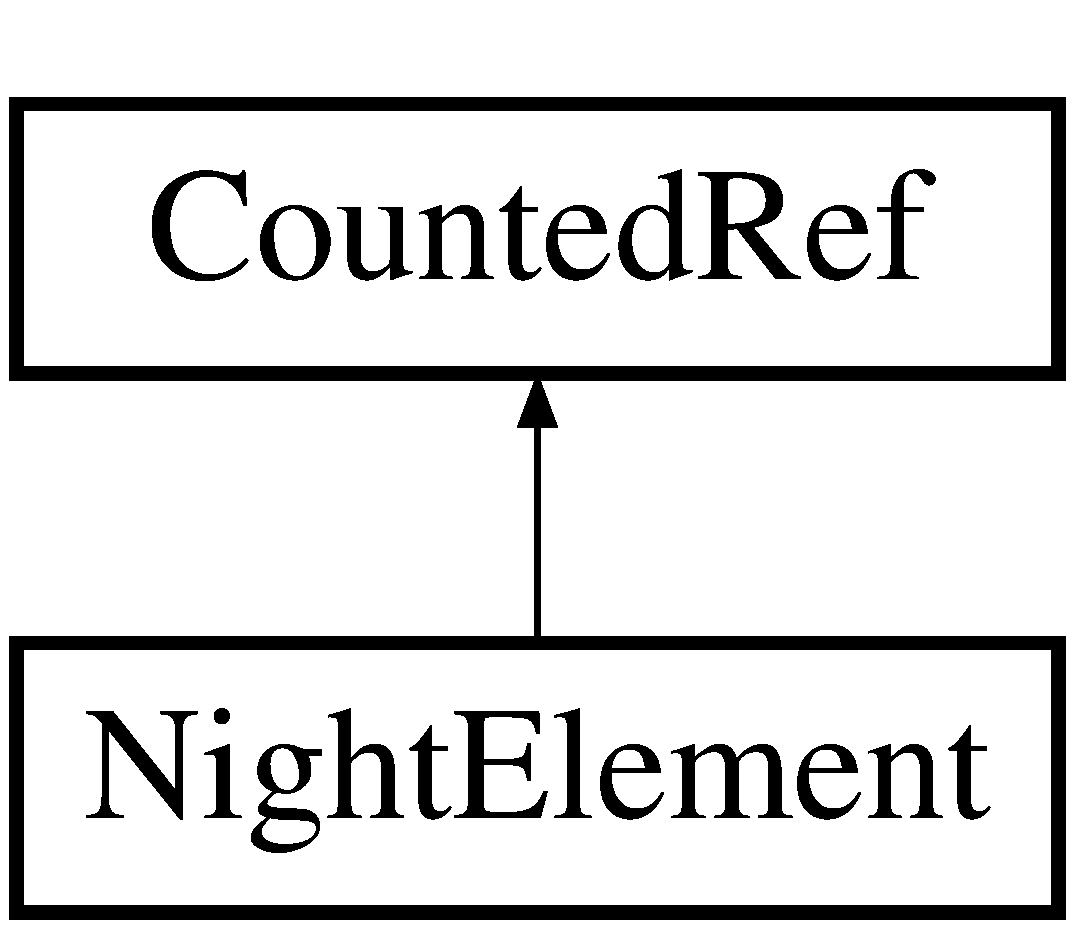
\includegraphics[height=2cm]{class_nightelement}
\end{center}
\end{figure}
\subsubsection*{Public Methods}
\begin{CompactItemize}
\item 
\index{NightElement@{NightElement}!NightElement@{Night\-Element}}\index{NightElement@{NightElement}!NightElement@{Night\-Element}}
{\bf Night\-Element} ()\label{class_nightelement_a0}

\begin{CompactList}\small\item\em empty constructor.\item\end{CompactList}\item 
\index{NightElement@{NightElement}!NightElement@{Night\-Element}}\index{NightElement@{NightElement}!NightElement@{Night\-Element}}
{\bf Night\-Element} (const Element \&An\-Element)\label{class_nightelement_a1}

\item 
\index{NightElement@{NightElement}!NightElement@{Night\-Element}}\index{NightElement@{NightElement}!NightElement@{Night\-Element}}
{\bf Night\-Element} (const {\bf Night} $\ast$ANight)\label{class_nightelement_a2}

\item 
\index{NightElement@{NightElement}!NightElement@{Night\-Element}}\index{NightElement@{NightElement}!NightElement@{Night\-Element}}
{\bf Night\-Element} (const Element \&An\-Element, const {\bf Night} $\ast$ANight)\label{class_nightelement_a3}

\item 
\index{~NightElement@{$\sim$NightElement}!NightElement@{Night\-Element}}\index{NightElement@{NightElement}!~NightElement@{$\sim$Night\-Element}}
{\bf $\sim$Night\-Element} ()\label{class_nightelement_a4}

\item 
\index{Clone@{Clone}!NightElement@{Night\-Element}}\index{NightElement@{NightElement}!Clone@{Clone}}
Night\-Element$\ast$ {\bf Clone} () const\label{class_nightelement_a5}

\end{CompactItemize}
\subsubsection*{Public Attributes}
\begin{CompactItemize}
\item 
\index{night@{night}!NightElement@{Night\-Element}}\index{NightElement@{NightElement}!night@{night}}
const {\bf Night}$\ast$ {\bf night}\label{class_nightelement_m0}

\end{CompactItemize}
\subsubsection*{Friends}
\begin{CompactItemize}
\item 
class {\bf By\-Increasing\-Seeing}
\item 
class {\bf By\-Increasing\-Time}
\end{CompactItemize}


\subsubsection{Detailed Description}
\subsubsection*{template$<$class Element$>$  class Night\-Element}

a template to use when an element belongs to a night.



The documentation for this class was generated from the following file:\begin{CompactItemize}
\item 
{\bf nightelement.h}\end{CompactItemize}
